\documentclass[12pt]{article}
\usepackage{../../template}
\author{niceguy}
\title{Lecture 18}
\begin{document}
\maketitle

\section{Hydrostataic Forces acting on Curved Surfaces}

Considering the same example

\begin{ex}

\begin{figure}
	\centering
	\caption{Gate}
	\label{gate}
	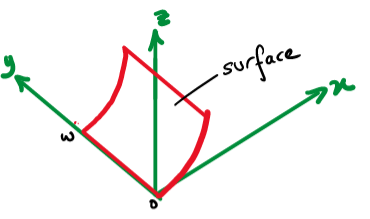
\includegraphics[width=0.7\textwidth]{gate.png}
\end{figure}

The surface is parametrised as

\begin{align*}
	x &= R\sin\theta \\
	z &= R - R\cos\theta \\
	y &= y
\end{align*}
so
$$\vec{r} = R\sin\theta\hat{i} + y\hat{j} + (R-R\cos\theta)\hat{k}$$
The moment is
\begin{align*}
	M &= \int d\vec{M} \\
	  &= \int \vec{r} \times d\vec{F} \\
	  &= -\int \vec{r} \times pd\vec{S}
\end{align*}

However, we only consider the moment about $y$, as the moments along the other axes are cancelled out by the hinge. Thus
$$dM_{\text{opening}} = ||d\vec{M}_y|| = (\vec{r}\times d\vec{S})\cdot\hat{j} (-p)$$
We have
\begin{align*}
	d\vec{S} &= \vec{r}_\theta \times \vec{r}_y \\
		 &= (R\cos\theta\hat{i} + R\sin\theta\hat{k}) \times \hat{j} \\
		 &= -R\sin\theta\hat{i} + R\cos\theta\hat{k}
\end{align*}
Then
\begin{align*}
	\vec{r} \times d\vec{S} &= (R\sin\theta\hat{i} + y\hat{j} + (R-R\cos\theta)\hat{k}) \times (-R\sin\theta\hat{i} + R\cos\theta\hat{k}) \\
				&= Ry\cos\theta\hat{i} - R^2\sin\theta\hat{j} + Ry\sin\theta\hat{k}
\end{align*}
Then the total moment is
\begin{align*}
	M_y &= \int_S dM_y \\
	    &= \int_0^{\frac{\pi}{2}} \int_0^w R^2\sin\theta \times \rho gR\cos\theta dyd\theta \\
	    &= \int_0^{\frac{\pi}{2}} \int_0^w \rho gR^3 \sin\theta\cos\theta d\theta dy
\end{align*}
where we again reach to the same integral.
\end{ex}

There is also another method, where one considers the free body diagram of the fluid. Consider the body $ABC$, where $AB$ represents the curve, and $AC$ and $BC$ are horizontal and veertical lines respectively. From equilibrium,

$$\sum F_x = 0 \Rightarrow F_{x,AB} = F_x$$
$$\sum F_y = 0 \Rightarrow F_{y,AB} = F_y + W$$

where $F_x$ is applied on $BC$ and $F_y$ on $AC$. Note the the direction of weight is reversed if the surface is above the liquid.

\begin{ex}
	Find the horizontal force $F$ required to hold the gate closed. Neglect the mass of the gate.

	\begin{figure}
		\centering
		\caption{Gate}
		\label{gate2}
		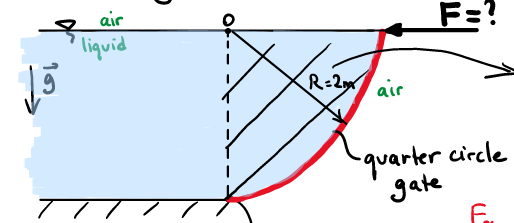
\includegraphics[width=0.7\textwidth]{gate2.png}
	\end{figure}

	Considering $\sum F_x = 0$, the horizontal component is
	$$F_x = \frac{1}{2}\rho g R^2w = 120000\text{N}$$
	Similarly for $y$,
	$$F_y = \rho g \frac{\pi R^2}{4}w = 60000\pi\text{N}$$
	Reaction force is
	$$\sqrt{F_x^2 + F_y^2} = 223451\text{N}$$
	at an angle
	$$\alpha = \arctan\left(\frac{F_y}{F_x}\right) = 57.5^\circ$$
	The perpendicular distance to the hinge is given by $R\cos\alpha$, so
	$$FR = 223451R\cos\alpha = 120000\text{N}$$
\end{ex}
\end{document}
